\documentclass{article}

%package setup
\usepackage{graphicx}
\usepackage{amsmath}
\usepackage{fancyhdr}
\usepackage[margin=1in]{geometry}
\usepackage{comment}
\usepackage{placeins}
\usepackage{parskip}
\usepackage{subcaption}
\usepackage{appendix}
\usepackage{soul}
\usepackage{comment}
\usepackage[hidelinks]{hyperref}
\usepackage{matlab-prettifier}
\usepackage{minted}
\usepackage{enumitem}
\usepackage{float}
\usepackage{textcomp, gensymb}

\pagestyle{fancy}
\fancyhf{} % Clear header/footer settings
\rhead{\thepage} % Page number on the right in the header
\lhead{ASE375 Lab Report 3} % Your lab report title on the left

\begin{document}

\begin{titlepage}
  \centering
  
\includegraphics[width=10cm]{ase-logo-formal.png}  % Adjust the width as needed
  \vspace{1cm}  % Add some vertical space
 
  \Large \textbf{ASE 375 Electromechanical Systems}\\
  \large \textbf{Section 14115}\\
  \vspace{0.5cm}
  \textbf{Monday: 3:00 - 6:00 pm}\\
 
  \vspace{1cm}
 
  \hrule
  \vspace{0.5cm}
 
  \Huge \textbf{Report 3:\\
  Measuring Displacement}\\
  \Huge \textbf{}\\
 
  \vspace{0.5cm}
  \hrule
 
  \vspace{1cm}
 
  \normalsize \textbf{Andrew Doty, Andres Suniaga, Dennis Hom}\\
  \normalsize \textbf{Due Date: 02/12/2024}
 
\end{titlepage}
\newpage

\tableofcontents
\thispagestyle{empty}
\newpage

\section{Introduction}
In this experiment we take a look at (1) Using a linear potentiometer to measure displacement of a small scale wing model with weights attached at different locations, (2) Determining the twist angle from these displacement measurements, and (3) Calculating the shear center, bending stiffness, and torsional stiffness of the wing model. 

This experiment attempts to accurately model measurements from the linear potentiometer in comparison to the ideal linear relationship from theoretical predictions. From these measurements we can then calculate the wing's shear center location and stiffness.  

\section{Equipment}
Devices used in this lab include:
\begin{itemize}

\item Digital Calipers: Used for measuring outer and inner dimensions of objects. In our case, digital calipers were used to measure the chord length of the small scale wing platofrm, the distance steps taken to calibrate the linear potentiometer, and the markings indicating chordwise locations for weight placement on the wing model.
\vspace{2.5mm}

\item Brass Slotted Weights with hanger: Used to induce bending on the wing model to acquire displacement measurements. Total $250$ grams.
\vspace{2.5mm}

\item LP804 Series Miniature Linear Potentiometer: Device used to measure linear position and displacement from wing bending and twisting.
\vspace{2.5mm}

\item 'Rare Earth' Magnets: High strength magnets used for secure placement of linear potentiometer to the wing platform to acquire measurements without slippage.
\vspace{2.5mm}

\item DAQ, NI-9215 Voltage Input Module, and LabVIEW: Data Acquisition System used to process data collected by digitizing the analog information into "bins" for a computer. NI-9215 used to measure the input voltage signals for the DAQ system. LabVIEW used to model voltages through the DAQ read from the linear potentiometer displacement.
\vspace{2.5mm}

\item Solderless Breadboard and Jumper Wires: Used to make connections from the linear potentiometer to power, ground, and signal for data collection.

\end{itemize}

\section{Procedure}
This section covers our procedure for this experiment broken into three parts. NOTE: For gathering measurements, ensure the standard deviation has reached a very small approximate steady-state and then mark down the LabVIEW output (upto the thousandth decimal digit).

\subsection{Calibration of Linear Potentiometer}
This first part contains our procedure for calibrating the linear potentiometer. Before beginning calibration, this part required connection setup of the linear potentiometer to the DAQ, NI-9215, and LabVIEW to collect and process data to model the input voltage measurements.

\begin{enumerate}
\item Ensure connection between the DAQ system (NI-9215) and the Linear Potentiometer is correct.
\vspace{2.5mm}

\item Take the potentiometer and place it on its side for better control of its displacement.
\vspace{2.5mm}

\item Using the digital calipers, measure from the base of the moving shaft on the linear potentiometer to the first displacement step $x_{1}$. We let the displacement step $\Delta x \approx 10\, mm$ for our calibration process. 
\vspace{2.5mm}

\item From the LabVIEW plot, gather the average voltage with the standard deviation for $x_{1}$. This will be a repeated process for each $x_{i}$.
\vspace{2.5mm}

\item Repeat the displacement and measurement process for $i>=5$ times, i.e. the next step is $x_{2} \approx 20\, mm$. We let $i = 6$ with an additional final calibration measurement $\approx 20\, mm$ from the $x_{6}$ step to cover the full range of the $5V$ input voltage.
\vspace{2.5mm}

\item We are now able to take the calibration data into Data Processing for plotting displacement $mm$ versus voltage $V$ to observe the linearity of the linear potentiomenter.

\end{enumerate}

\subsection{Chordwise Displacement}
This is Part 1 of measuring displacements from weights attached to our wing model. Enusre proper setup of the linear potentiometer under the wing platform to begin displacement measurement at different chordwise locations.
\begin{enumerate}
  \item With the digital caliper, measure the chord length of the wing model. With the caliper, make $n>=10$ markings for chordwise locations between $0$ and $c$ (chord). For our setup, we marked chordwise locations $y_{c} \approx \left[0,\, 10,\, 20,\, 30,\, 40,\, 50,\, 60,\, 70,\, 80,\, 90,\, 100\right]\, mm$, from trailing edge to leading edge.
  \vspace{2.5mm}
  
  \item Place a 'rare earth' magnet to either the leading edge or trailing edge joint and secure the tip of the potentiometer to that joint.
  \vspace{2.5mm}

  \item Hang the weight ($250$ grams in our setup) to the first chordwise position and gather the average voltage with the standard deviation from the LabVIEW model. This will be used to process displacement measurement.
  \vspace{2.5mm}

  \item Repeat step (3) through each $y_{c}$ element and mark down the measurements for each position.
  \vspace{2.5mm}

  \item Once finished with measurements at the first edge, switch to the other edge and follow steps (3) and (4) again. For example, if leading edge was chosen first, position the magnet and potentiomenter to the trailing edge joint next.
  \vspace{2.5mm}

  \item After finishing these procedure, take measurements into Data Processing for determining the Shear Center location of the wing model.
\end{enumerate}

  \subsection{Spanwise Displacement}
  Part 2 of displacement measurements involve measuring spanwise displacement due to weight hanging at three different trailing edge joints throughout the span of the wing platform. Ensure proper setup of linear potentiomenter under the span of the wing platform. 
  % \begin{figure}
  %   \centering
  %   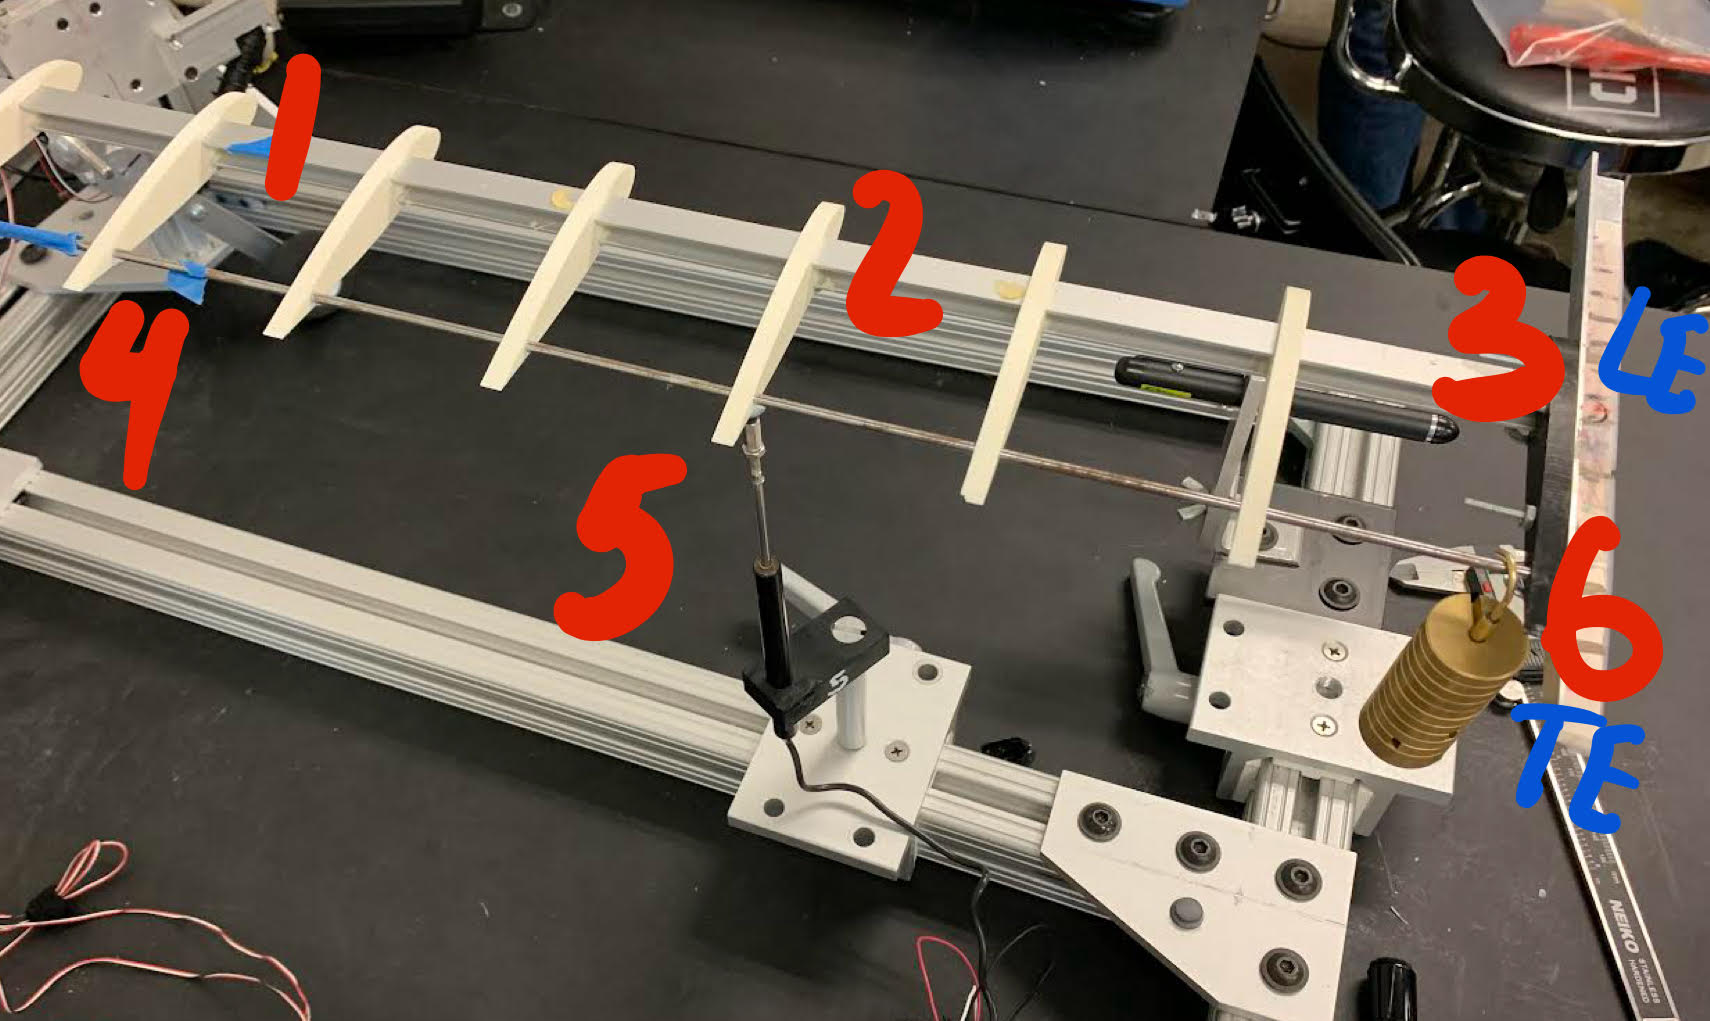
\includegraphics[width = \textwidth]{lab3images/SpanwiseLocations.jpg}
  %   \caption{Spanwise position indexing with Leading and Trailing Edge labels}
  % \end{figure}
  
  \begin{enumerate}
    \item Start by hanging the weight at the $6^{th}$ position as shown in \textbf{Figure (1)}. 
    \vspace{2.5mm}

    \item Place the magnet and potentiomenter at a spanwise location of choice and gather the input voltage measurement along with the standard deviation.
    \vspace{2.5mm}

    \item Repeat (2) measurements for all other spanwise locations.
    \vspace{2.5mm}

    \item Next, move the weight to the $5^{th}$ position.
    \vspace{2.5mm}
  \end{enumerate}

\section{Data Processing}
\subsection*{Variables}
\begin{enumerate}[label = \roman*.]
  \item (\(EI\)): Bending Stiffness
  \item (\(GJ\)): Torsional Stiffness
  \item (\(e\)): Location of Shear Center
  \item (\(S_{j}\)): Shear Force at a \(j\) coordinate
  \item (\(x_{j}\)): Spanwise coordinate
  \item (\(y_{f}\)): Chordwise Coordinate
  \item (\(M_{j}\)): Moment acting at \(j\) coordinate
  \item (\(\tau_{j}\)): Torque acting at \(j\) coordinate
\end{enumerate}

\subsection*{Equations}
\begin{enumerate}[label = \Roman*.]
    \item 
\end{enumerate} 


\section{Results and Analysis}

\begin{table}[hbtp]
  \centering
  \begin{tabular}{|c|c|c|c|c|c|c|c|}
  \hline
  X-pos. & LE Volt \(V\) & LE STD & LE Def. \(mm\) & TE Volt \(V\) & TE STD & TE Def. \(mm\) & Theta \(rad\) \\
  \hline
  0 & 2.014 & 0.00096 & 29.2859375 & 1.948 & 0.00093 & 28.2546875 & -0.010230298 \\
  10 & 2.014 & 0.00096 & 29.2859375 & 1.966 & 0.00099 & 28.5359375 & -0.007440339 \\
  20 & 2.005 & 0.00096 & 29.1453125 & 1.986 & 0.00095 & 28.8484375 & -0.00294518 \\
  30 & 2.004 & 0.00095 & 29.1296875 & 2.002 & 0.001 & 29.0984375 & -0.00031002 \\
  40 & 1.99 & 0.00096 & 28.9109375 & 2.029 & 0.00093 & 29.5203125 & 0.006045313 \\
  50 & 1.997 & 0.001 & 29.0203125 & 2.058 & 0.001 & 29.9734375 & 0.009455323 \\
  60 & 1.993 & 0.00099 & 28.9578125 & 2.081 & 0.00099 & 30.3328125 & 0.013640027 \\
  70 & 1.985 & 0.00097 & 28.8328125 & 2.108 & 0.00098 & 30.7546875 & 0.01906391 \\
  80 & 1.9898 & 0.00099 & 28.9078125 & 2.136 & 0.00097 & 31.1921875 & 0.022658572 \\
  90 & 1.988 & 0.001 & 28.8796875 & 2.165 & 0.001 & 31.6453125 & 0.027429874 \\
  100 & 1.979 & 0.00098 & 28.7390625 & 2.186 & 0.00096 & 31.9734375 & 0.032076048 \\
  \hline
  \end{tabular}
  \caption{Leading and Trailing Edge Data}
  \label{tab:LE_TE_Data}
\end{table}
  
\begin{table}[hbtp]
  \centering
  \begin{tabular}{|c|c|}
  \hline
  Weight \(kg\) & 0.25 \\
  \hline
  Shear Force \(N\) & 2.4525 \\
  \hline
  Shear Center & 0.31\% Chord \\
  \hline
  Moment \(N*cm\) & 67.44375 \\
  \hline
  Torque \(N*mm^2\) & 170.57628 \\
  \hline
  Deflection \(X_i=11\) & 4004.091667 \\
  \hline
  Deflection \(X_i=19.25\) & 11753.00729 \\
  \hline
  Deflection \(X_i=27.5\) & 22945.88542 \\
  \hline
  EI \(N*m^2\) & 490.5 \\
  \hline
  GJ \(N*m\) & 213.22035 \\
  \hline
  \end{tabular}
  \caption{Deflection and Stiffness Data}
  \label{tab:deflect_stiff}
\end{table}

\begin{table}[hbtp]
  \centering
  \begin{tabular}{ccccc}
  \hline
  Leading Edge & Deflection & Trailing Edge & Deflection & Theta \\
  \hline
  48.895 & 32.7234375 & 48.895 & 36.8953125 & 0.041364042 \\
  69.85 & 36.4265625 & 69.85 & 41.7078125 & 0.052345491 \\
  27.94 & 28.8796875 & 27.94 & 30.6609375 & 0.017669292 \\
  48.895 & 33.9421875 & 48.895 & 38.4265625 & 0.044458532 \\
  69.85 & 37.8796875 & 69.85 & 43.1921875 & 0.052654657 \\
  \hline
  \end{tabular}
  \caption{Actual Deflection}
  \label{table:actual_deflection}
  \end{table}
  
As for our uncertainty, we can use the least count of our different measuring devices as a basis for the overall uncertainty. That gives us the following equation:
\[
\delta_{\text{total}} = \sqrt{\delta_{\text{caliper}}^2 + \delta_{\text{potentiometer}}^2 + \delta_{\text{DAQ}}^2}
\]

In this case, the caliper or ruler measurements are accurate to the nearest millimeter, the potentiomenter is accurate to the nearest hundredth of a millimeter, and the DAQ is accurate to the nearest thousandth of a volt. This gives us the following uncertainties: 
\begin{itemize}
  \item Caliper: \(\delta_{\text{caliper}} = 0.5\, \text{mm}\)
  \item Potentiometer: \(\delta_{\text{potentiometer}} = 0.005\, \text{mm}\)
  \item DAQ: \(\delta_{\text{DAQ}} = 0.001\, \text{V}\)
\end{itemize}

For our overall propagation of uncertainty, we have:
\[
\delta_{\text{total}} = \sqrt{0.5^2 + 0.005^2 + 0.001^2} = 0.501\, \text{mm}
\]
Graphically, our results are as follows.


\begin{figure}[hbtp]
  \centering
  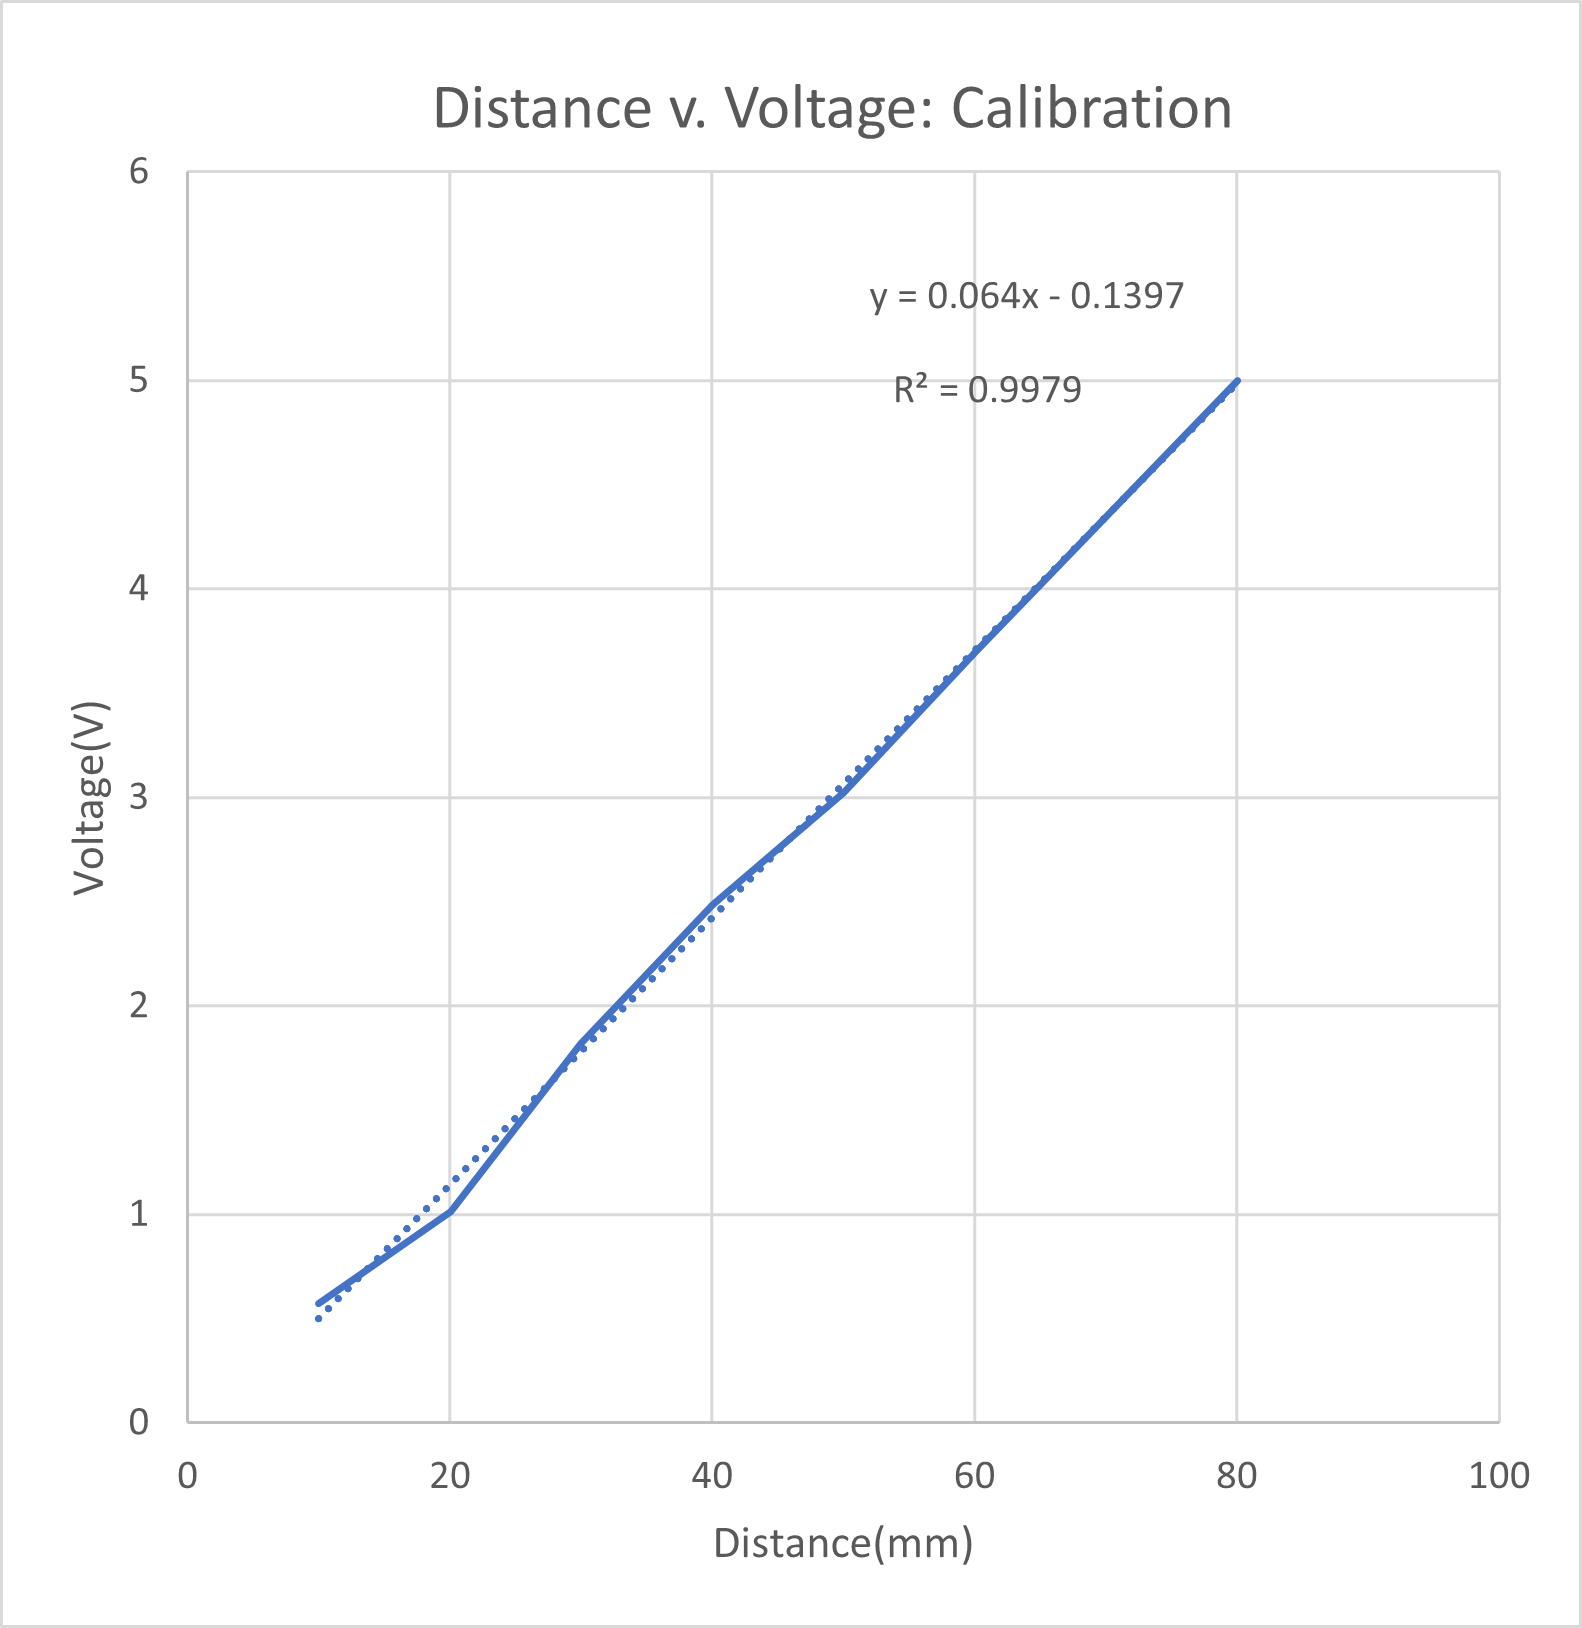
\includegraphics[width=0.95\textwidth]{lab3images/Calibration.png}
  \caption{Calibrating our Linear Potentiometer}
  \label{fig:Calibration}
\end{figure}


\begin{figure}[hbtp]
  \centering
  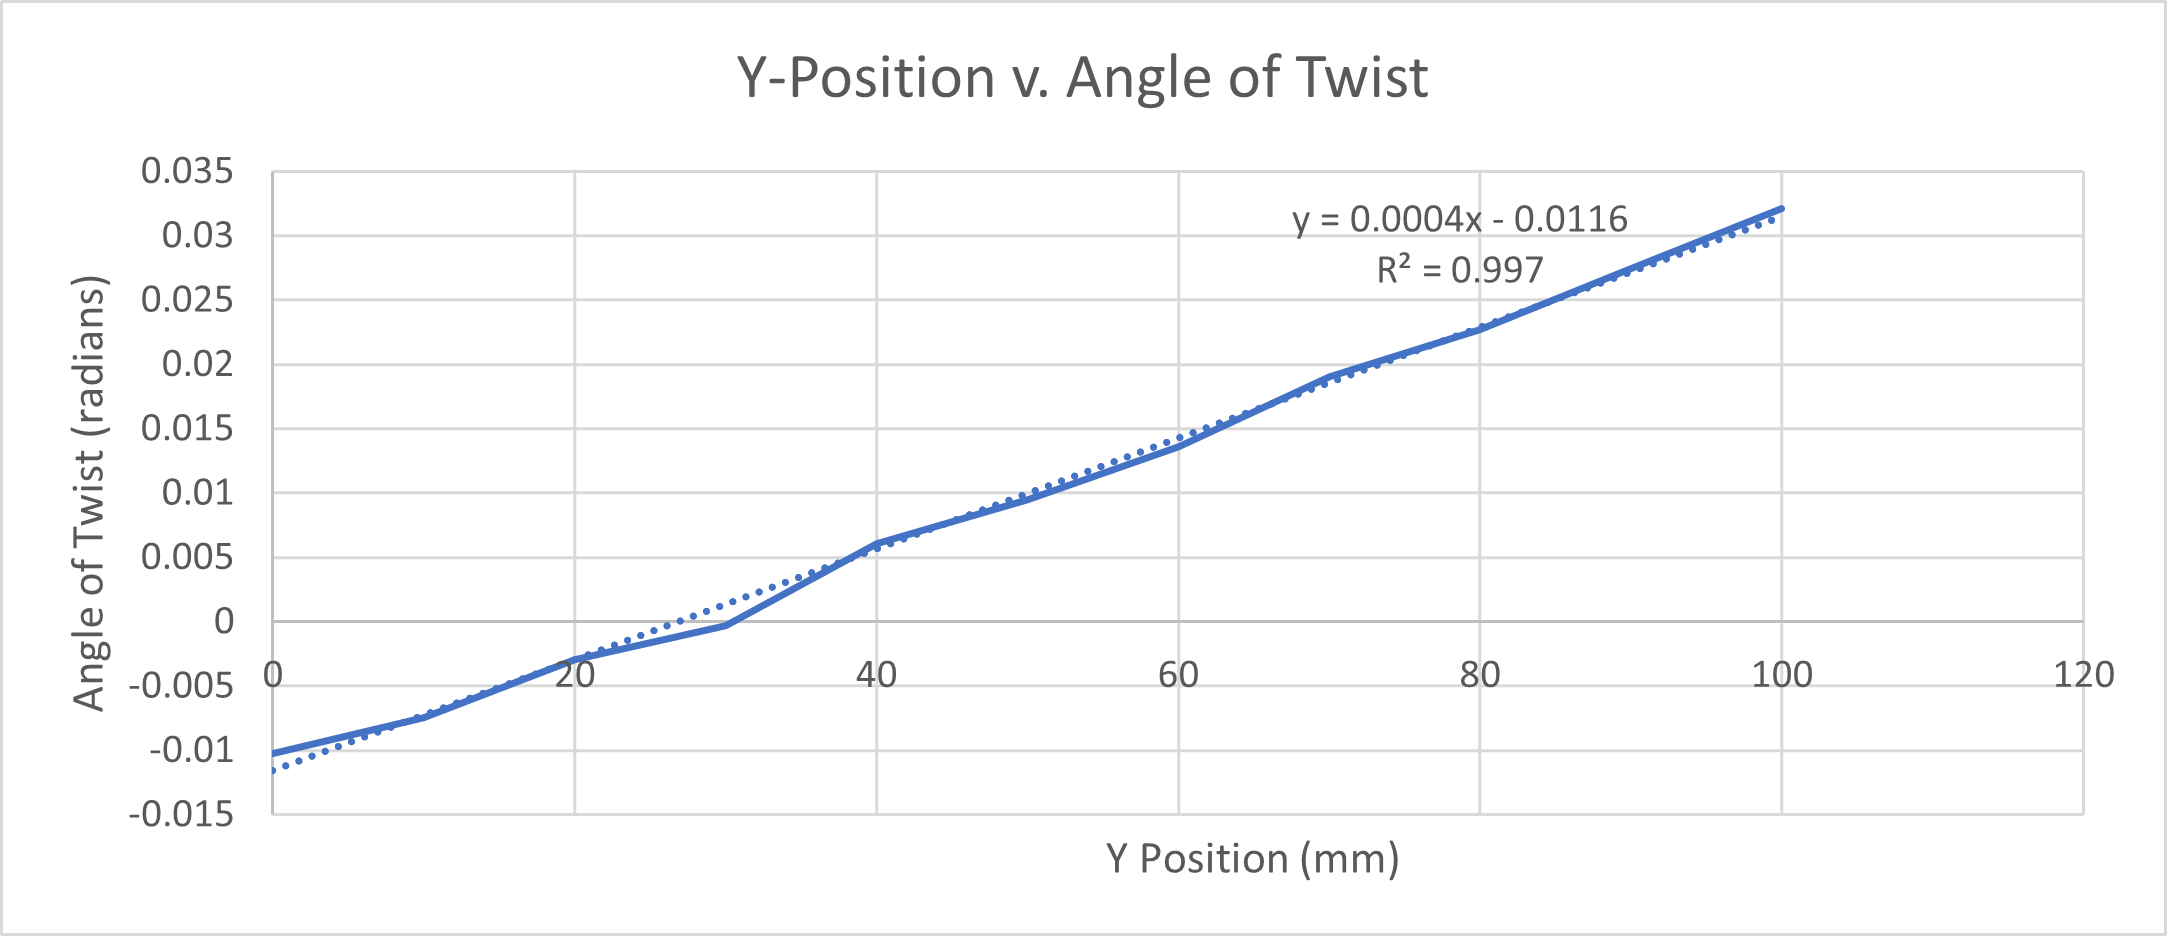
\includegraphics[width=0.95\textwidth]{lab3images/YvsTwist.png}
  \caption{Y distance vs Twist Angle}
  \label{fig:YvsTwist}
\end{figure}


\begin{figure}[hbtp]
  \centering
  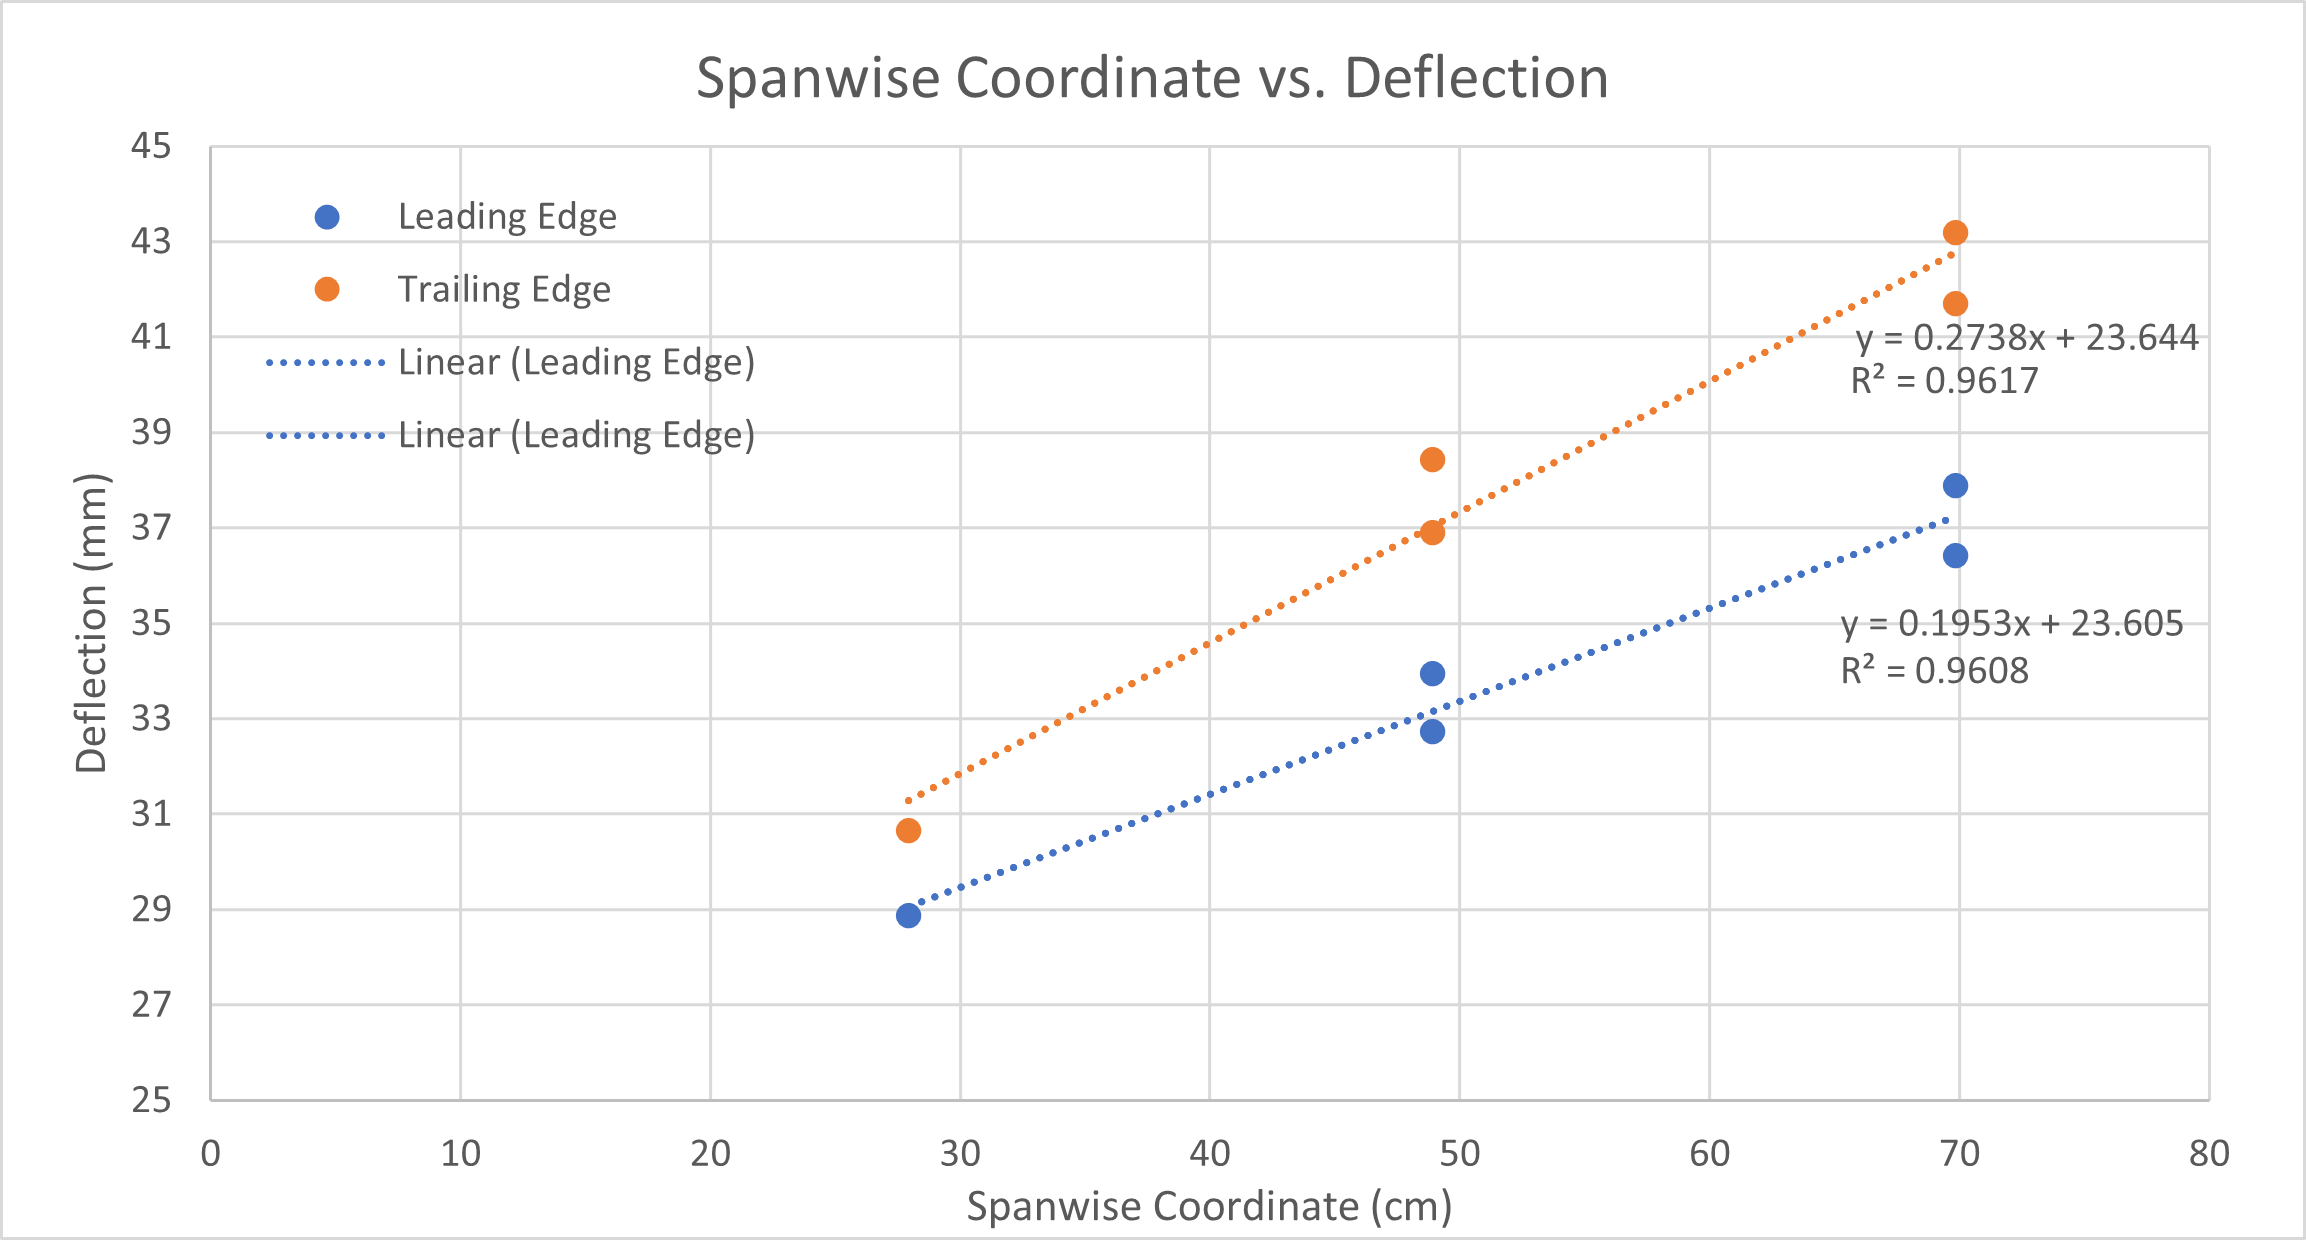
\includegraphics[width=0.95\textwidth]{lab3images/SpanwiseDeflection.png}
  \caption{Spanwise Coordinates vs Deflection with varying weight placement}
  \label{fig:SpanwiseDeflection}
\end{figure}


\section{Conclusion}

\newpage
\thispagestyle{empty}  % Clear header/footer
\begin{center}
	\vspace*{\fill}
	{\Huge Appendices}
	\vspace*{\fill}
\end{center}

% Start appendices
\newpage
\begin{appendices}
\pagestyle{fancy}
\renewcommand{\thefigure}{A\arabic{figure}}
\setcounter{figure}{0}

\section*{Appendix: t-Distribution Tables}
\hypertarget{1}{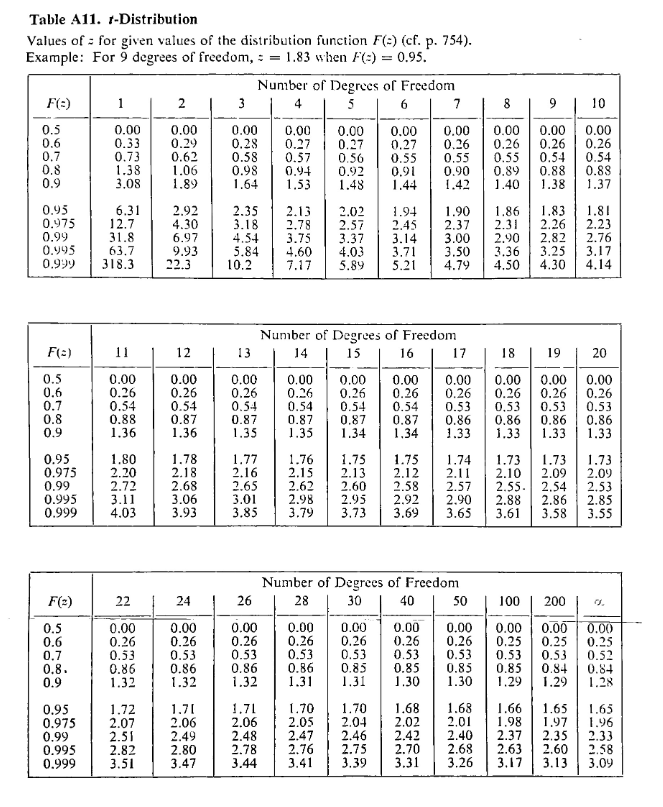
\includegraphics[width=0.95\textwidth]{t_distribution_Table_lecture3.png}}
\end{appendices}

\end{document}
